%% Supplementary Material of Paper 1. The settings and grounds that Section 3 of
%% the main text gives in one clause are stated here in full; section numbers
%% S1 to S6 are cited from the main text.
\documentclass[12pt]{article}
\usepackage[T1]{fontenc}
\usepackage[utf8]{inputenc}
\usepackage{lmodern}
\usepackage{amsmath,amssymb}
\usepackage{booktabs}
\usepackage{graphicx}
\graphicspath{{figures/}}
\usepackage{float}
\usepackage{siunitx}
\usepackage[margin=2.5cm]{geometry}
\usepackage[authoryear,round,semicolon]{natbib}
\usepackage[hidelinks]{hyperref}
\usepackage{microtype}

\renewcommand{\thesection}{S\arabic{section}}
\renewcommand{\thetable}{S\arabic{table}}
\renewcommand{\thefigure}{S\arabic{figure}}

\title{Supplementary Material\\[0.4em]
\large Relative effects of seagrass canopy, wave coupling and bed mobility on
Lagrangian transport in a shallow lagoon}
\author{Cicero Martins Jr., Mauro De Marchis, Giuseppe Ciraolo,\\
Carmelo Nasello, Antonino Maltese}
\date{}

\begin{document}
\maketitle

\section{Hydrodynamic model settings}
\label{sec:s_model}

The computational mesh comprised 21{,}188 nodes and 25{,}212 faces, 14{,}969
of them quadrilateral and 10{,}243 triangular, spanning 11.96--12.56$^\circ$E
and 37.70--38.06$^\circ$N in geographic (WGS84) coordinates. Taking the
distance between the centres of adjacent wet cells as the measure of
resolution, the mesh grades from about 880~m in the open offshore to about
60~m in the lagoon and in the bands that follow the Egadi and mainland
shorelines (Fig.~\ref{fig:s_mesh}). The constraint the grading answers is the width of the inlets,
which carry the exchange that sets the interior response. At the 61~m median
spacing around the northern inlet, about six cells span its 400~m width, and
about forty span the 2900~m southern inlet, while the 20~m dredged channel
through the northern sill falls below the mesh scale and enters only through
the cell-centre bathymetry.

\begin{figure}[H]
  \centering
  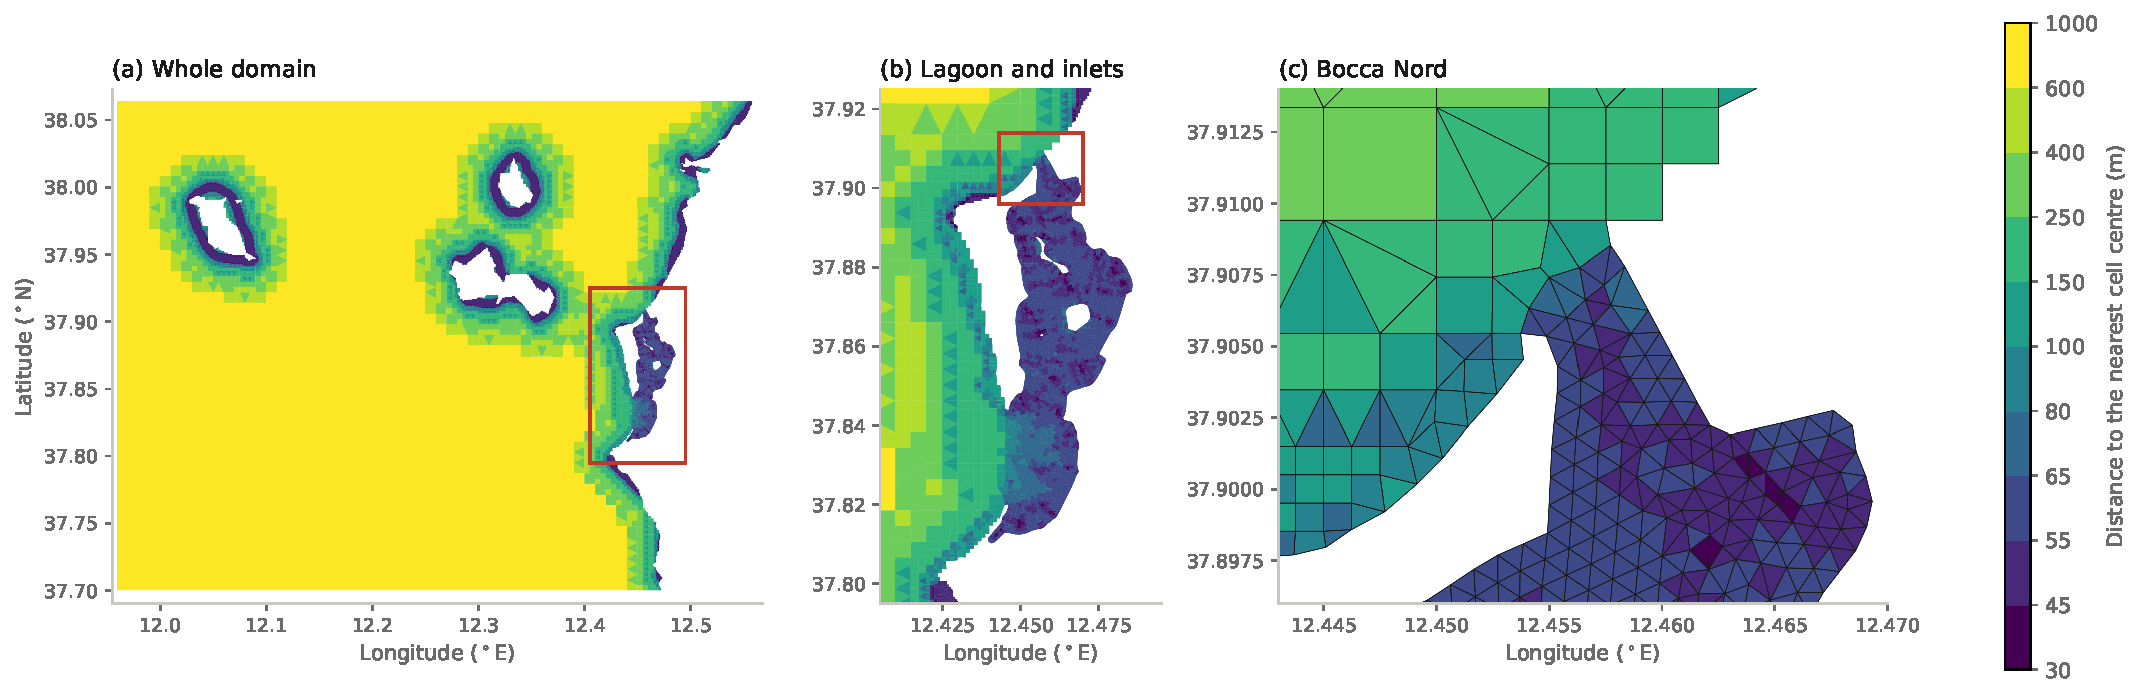
\includegraphics[width=\textwidth]{figS1}
  \caption{Resolution of the hydrodynamic mesh, given as the distance from each
  cell centre to the nearest neighbouring cell centre, over (a) the whole
  domain, (b) the lagoon and its inlets and (c) the northern inlet, Bocca Nord,
  with the cell edges drawn. The boxes in (a) and (b) mark the extent of the
  next panel.}
  \label{fig:s_mesh}
\end{figure}

The 10 uniform sigma layers answer two features of the problem, since resolving
the wind-driven surface drift over a near-bed return flow requires several
layers through a sub-metre column, and the 0.40~m canopy spans the lowest four
of the ten layers and part of the fifth at the mean depth, so that its drag is
distributed over the vertical rather than collapsed into a single near-bed term.

Momentum advection used the Perot scheme with a monotone central limiter on
the cell-centre velocity, and the same limiter was applied to the transport of
salinity and temperature. The water-level system was solved with a
preconditioned conjugate-gradient method. Bed levels were specified at cell
centres from the bathymetry file.

Turbulence closure used the $k$--$\varepsilon$ model with background vertical
eddy viscosity and diffusivity of $10^{-4}$~\si{\metre\squared\per\second} and
uniform horizontal values of 0.1~\si{\metre\squared\per\second}. Density was
computed from the UNESCO equation of state, with salinity and temperature both
transported as active constituents so that the summer hypersaline gradient
contributes baroclinically to the momentum balance.

External forcing was updated every 300~s, shorter than the interval of every
forcing record used, so the update does not set the time resolution of the
forcing. The computational time step was adaptive under a Courant limit of 0.7
and capped at 30~s in the members coupled to the wave model and at 15~s in the
uncoupled ones, at least an order of magnitude below the forcing update so that
no forcing interval is crossed in a single step, and constrained to grow by no
more than a factor 1.1 between successive steps, which keeps the step from
recovering abruptly after the wetting and drying events on the intertidal flats
where the Courant limit binds. Initial conditions were ramped over the first
hour.

The domain was decomposed into eight partitions and run under MPI. Eight
partitions leave about 3000 cells each, above the few thousand below which the
communication cost of the parallel solver begins to dominate for meshes of this
size \citep{Moge2019}. All members were run on the same 48-core Linux server
with the same decomposition, where a coupled nine-day member completed in four
and a half to six hours of wall-clock time and an uncoupled member in under
three.

\section{Wave model settings}
\label{sec:s_waves}

The outer grid, $69 \times 54$ points at approximately 800~m, covered the full
flow domain and took its boundary spectra from the western, southern and
northern edges, and it supplied boundary conditions to an inner grid of
$121 \times 221$ points at 88~m east--west and 111~m north--south over the
lagoon and its inlets. The outer grid matches the 880~m background of the
hydrodynamic mesh offshore. The inner grid is 1.5 to 1.8 times coarser than the
60~m flow mesh inside the lagoon, spanning the 400~m northern inlet with about
four cells against the flow mesh's six, so the wave field is the coarser of
the two representations of the inlets and is interpolated onto a finer flow
mesh (Fig.~\ref{fig:s_swan}). Table~\ref{tab:swan} lists the
settings and their grounds.

\begin{figure}[H]
  \centering
  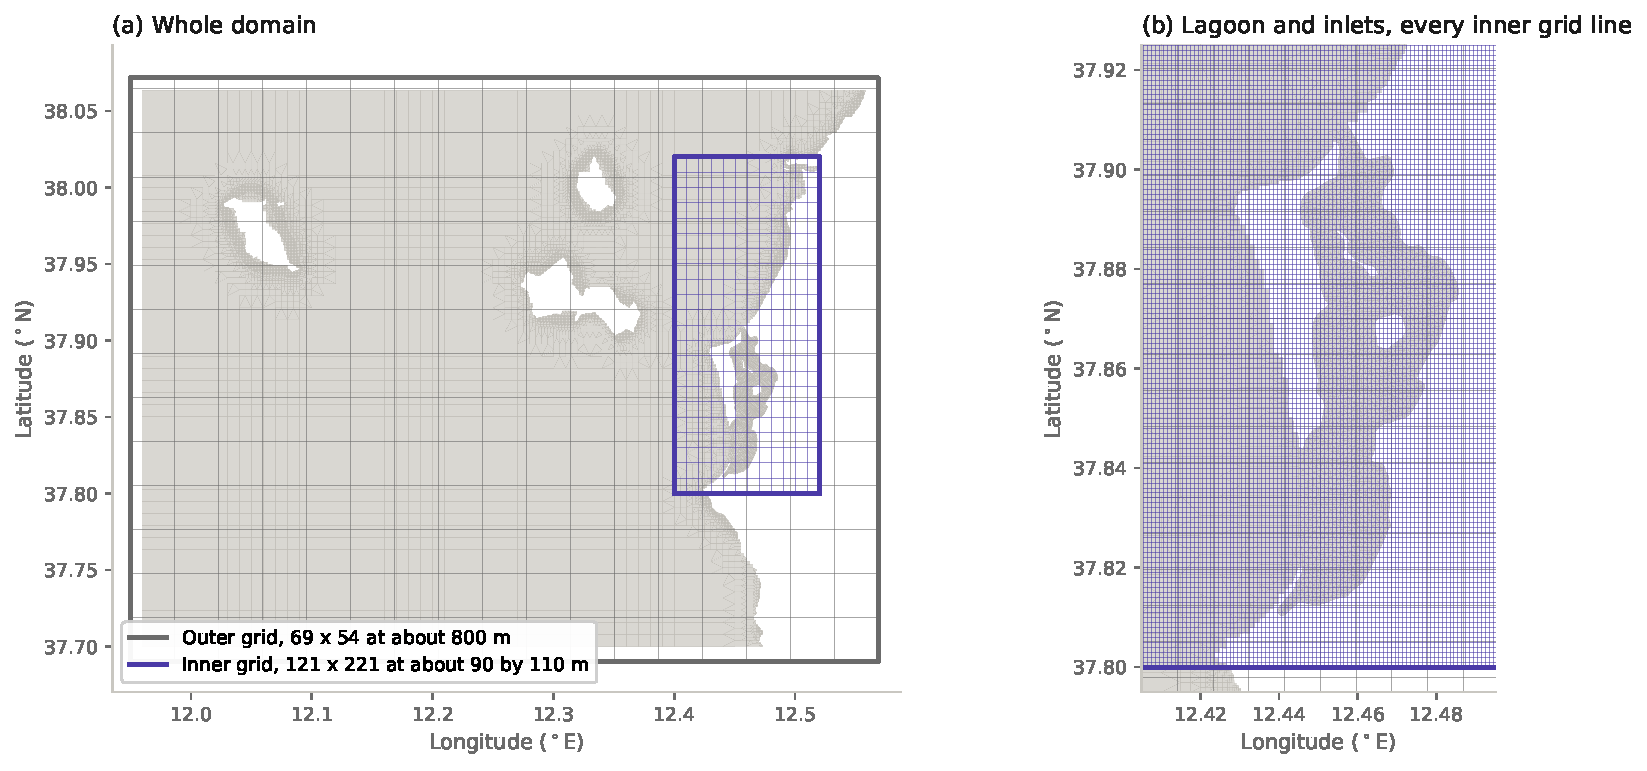
\includegraphics[width=\textwidth]{figS2}
  \caption{SWAN computational grids over the hydrodynamic mesh, in grey. (a)
  Outer grid of $69 \times 54$ points and inner grid of $121 \times 221$
  points nested over the lagoon, with every fourth line of the outer grid and
  every tenth line of the inner grid drawn. (b) Lagoon and inlets, with every
  line of the inner grid drawn.}
  \label{fig:s_swan}
\end{figure}

\begin{table}[H]
  \centering
  \caption{SWAN settings and the ground for each.}
  \label{tab:swan}
  \small
  \begin{tabular}{p{0.30\textwidth}p{0.62\textwidth}}
    \toprule
    Setting & Ground \\
    \midrule
    24 directions over the full circle (15$^\circ$) & Standard directional resolution \\
    24 frequencies, logarithmic, 0.05--1.0~Hz & Periods of 1 to 20~s bracket the swell entering through the inlets and the short waves of the basin, whose fetch-limited peak period over the 2.5~km cross-basin fetch is of the order of 2~s \\
    Third generation, Komen whitecapping, quadruplets, refraction, frequency shifting & Standard set for a wind-sea dominated application \\
    Triad interactions off & They redistribute energy within the spectrum in very shallow water, and the quantity exchanged with the flow solver is the depth-integrated dissipation rather than the spectral shape \\
    Wave setup off & The free surface is computed by the flow solver, which already receives the wave forcing, so setup in the wave model would apply that contribution twice \\
    Depth-induced breaking, \citet{BattjesJanssen1978}, $\alpha = 1.0$, $\gamma = 0.73$ & $\gamma$ is the mean value of \citet{BattjesStive1985} over laboratory and field data \\
    JONSWAP bottom friction, 0.067~\si{\metre\squared\per\cubic\second} & Value for wind sea rather than the lower value appropriate to swell \citep{BouwsKomen1983} \\
    Minimum depth 0.05~m & Excludes the thin films on the intertidal flats, where the spectral formulation carries no meaning \\
    Stationary mode, convergence at 2\% of $H_s$ and $T_m$ at 98\% of wet points, at most 15 iterations & See text \\
    Exchange every 3600~s through DIMR & See text \\
    Communication files in classic NetCDF (\texttt{ncFormat = 3}) & Required for the wave module to re-open the communication file reliably across the coupled run \\
    \bottomrule
  \end{tabular}
\end{table}

The exchange interval was set by the time scales the coupling has to resolve,
the 12.4~h tide and the diurnal sea breeze, and by cost, the wave model
accounting for about four fifths of the wall time of a coupled run. It bounds
the time resolution of the wave field, and since the drifter deployments last
between 0.4 and 7.2~h, the shortest of them are advected through a single wave
field.

Within each exchange the wave model ran in stationary mode, so the time
variation of the wave field followed from the re-evaluated water levels,
currents, wind and boundary spectra rather than from spectral propagation in
time. The assumption is that the wave field equilibrates with its forcing
faster than the forcing changes. Inside the lagoon, where the fetch is at most
2.5~km across the basin and the depth is of order 1~m, wave energy crosses the
generation area in about fifteen minutes at the shallow-water group velocity,
well within the hourly exchange. Offshore the crossing time is longer, but the
sea state there is prescribed from the boundary spectra rather than generated
inside the domain.

\section{Boundary offset, initial condition and atmospheric forcing}
\label{sec:s_forcing}

The per-node offset added to the water-level boundary is anchored on the tide
gauge at Marettimo island (JRC TAD 658) and distributed along the boundary
using the CMEMS mean dynamic topography. The anchor is the mean difference
between the gauge record and the CMEMS field interpolated to the gauge, both
reduced to daily means, over 384 aligned days spanning January 2025 to January
2026. It amounts to $+0.449$~m, of which the gauge contributes $+0.091$~m and
the CMEMS rest-state reference the remaining $-0.358$~m. The monthly means of
that difference range from $+0.361$ to $+0.505$~m, so a seasonal residual of
about 0.07~m either side of the annual value is not removed by a constant
anchor, which bounds the accuracy of the reference level the model can be held
to (Fig.~\ref{fig:s_offset}).

\begin{figure}[H]
  \centering
  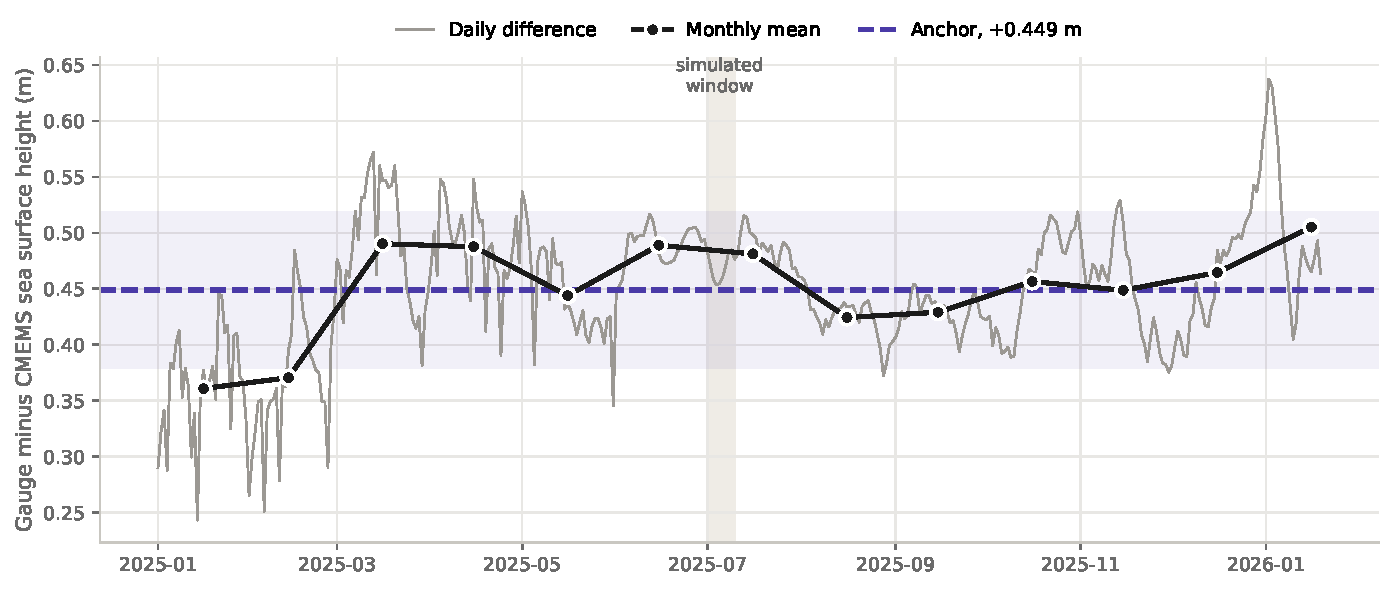
\includegraphics[width=\textwidth]{figS3}
  \caption{Difference between the water level at the Marettimo gauge and the
  CMEMS sea surface height interpolated to the gauge, as daily means over the
  384 aligned days, with the monthly means and the mean of $+0.449$~m taken as
  the anchor of the boundary offset. The horizontal band spans 0.07~m either
  side of the anchor, and the vertical band marks the simulated window.}
  \label{fig:s_offset}
\end{figure}

The stratified start takes the CMEMS temperature and salinity profiles at the
start time and applies them over the domain outside the lagoon, while the
uniform start holds the whole column at 24~$^\circ$C and 37.5
(Fig.~\ref{fig:s_ic}). Over the lagoon both starts carry the hypersaline value
of 42. The two profiles differ most in the upper 50~m, where the CMEMS
temperature falls from 25.8 to 17.6~$^\circ$C and the salinity passes
through a minimum of 37.33 at about 22~m.

\begin{figure}[H]
  \centering
  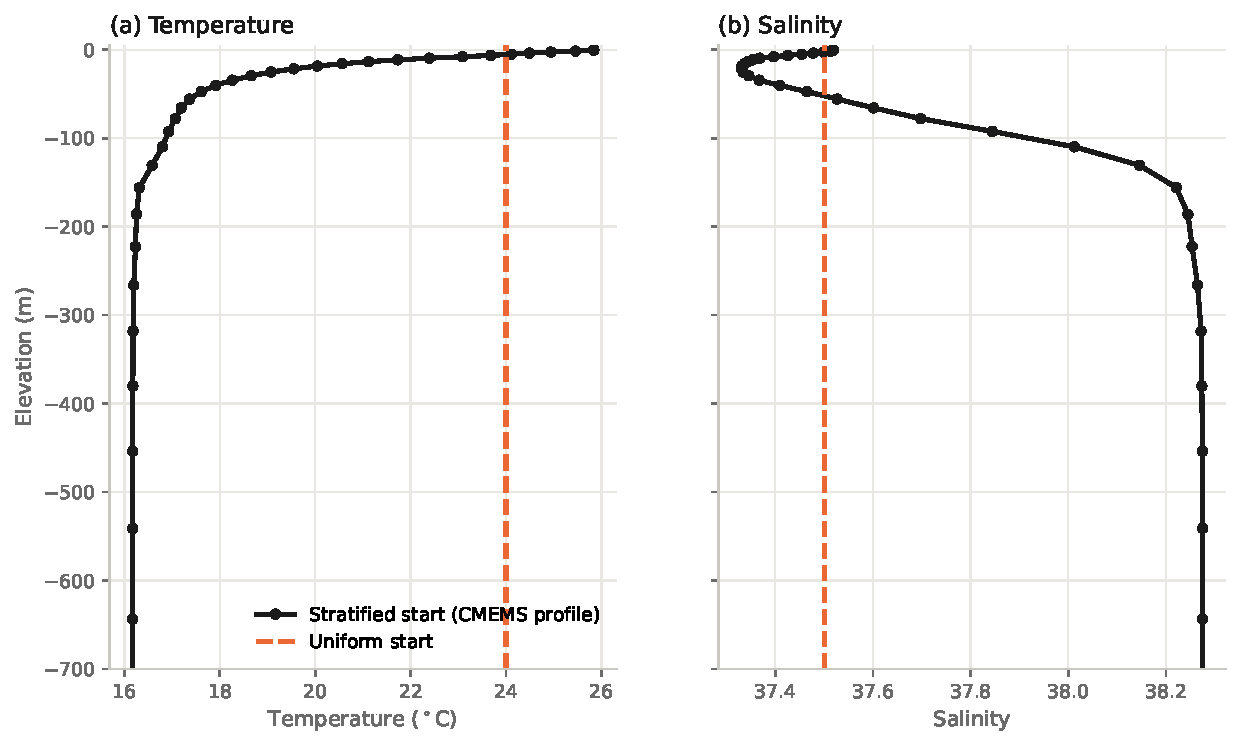
\includegraphics[width=0.85\textwidth]{figS4}
  \caption{Initial (a) temperature and (b) salinity outside the lagoon, as the
  CMEMS profile used by the stratified start and the vertically uniform values
  of the uniform start.}
  \label{fig:s_ic}
\end{figure}

The wind field was blended with the record of the AltaVilaEst station alone.
Configurations that additionally blended a second in-situ station produced a
systematic rotation of the wind vector along the eastern lagoon margin. The
hourly ERA5 field was interpolated to a 0.005$^\circ$ grid and combined with
the hourly mean of the station record through a weight that depends on the
distance from the lagoon centre, equal to one within 3~km, which covers the
central basin and the station, and decreasing linearly to zero at 8~km, beyond
which ERA5 applies unchanged, so that the northern and southern ends of the
lagoon, 4 to 7~km from the centre, carry a mixture of the two (Fig.~\ref{fig:s_wind}). Over the
simulation window the station recorded a mean speed of 4.5~m~s$^{-1}$ against
3.3~m~s$^{-1}$ for ERA5 at the lagoon centre, with a median absolute
difference in direction of 17$^\circ$. During the drifter campaign the two
means were 6.6 and 5.5~m~s$^{-1}$ and the median difference in direction
11$^\circ$.

\begin{figure}[H]
  \centering
  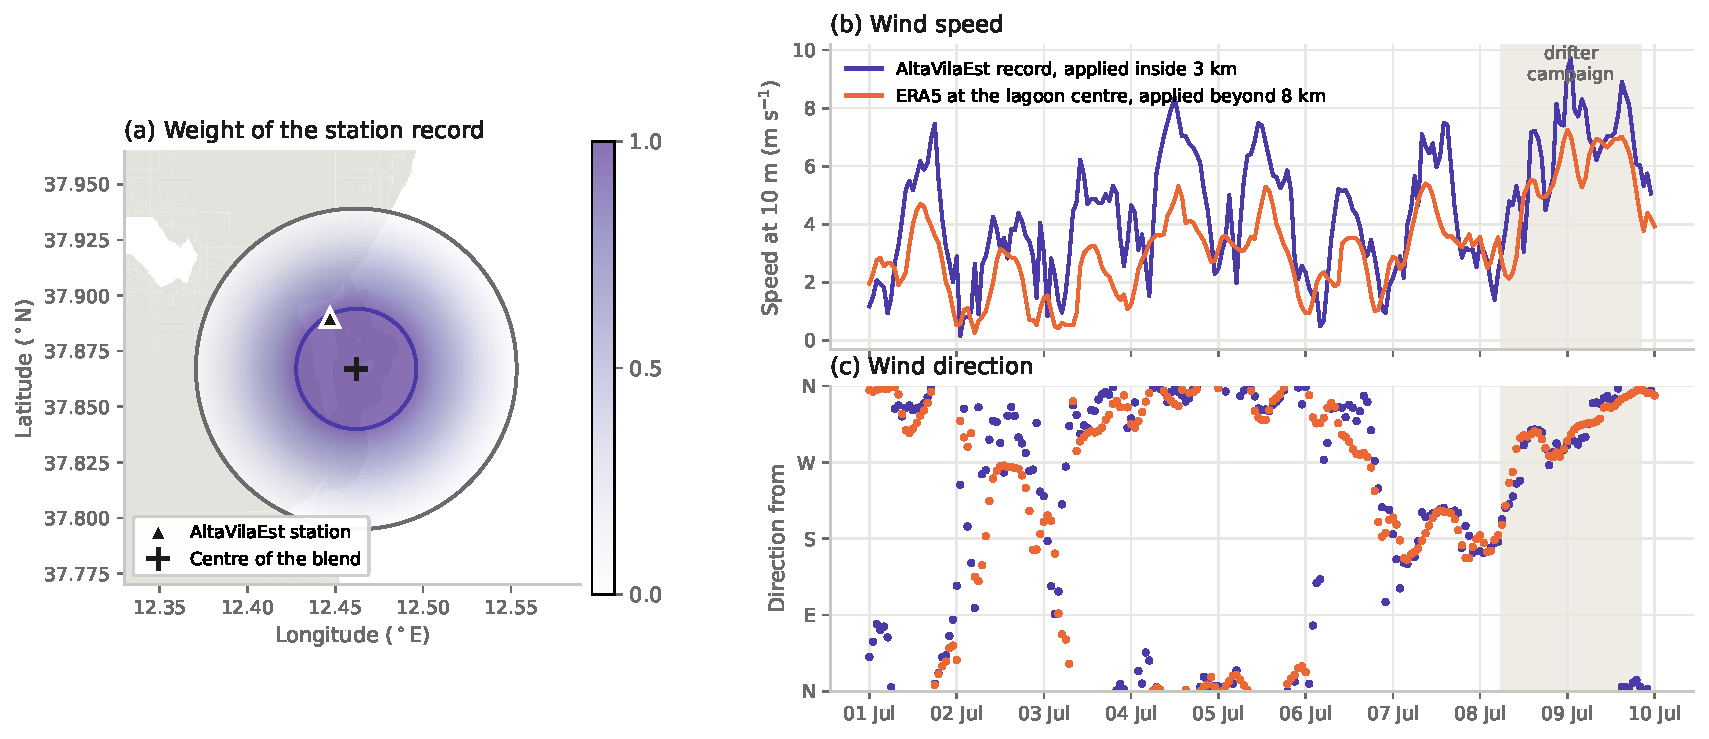
\includegraphics[width=\textwidth]{figS3_wind}
  \caption{Wind forcing. (a) Weight of the AltaVilaEst record in the blended
  field, with the circles of 3 and 8~km around the lagoon centre. (b) Hourly
  wind speed and (c) direction from which the wind blows, at the AltaVilaEst
  station and in ERA5 at the lagoon centre, with the drifter campaign shaded.}
  \label{fig:s_wind}
\end{figure}
Evaporation was imposed through the rainfall quantity with a negative sign,
which is the convention D-Flow FM expects, with both the rainfall and
evaporation switches enabled in the model definition.

\section{Canopy parameters and seagrass classification}
\label{sec:s_canopy}

Densities are expressed per leaf rather than per shoot, since it is the leaf
that presents the frontal area and \emph{P.\ oceanica} carries about six leaves
per shoot \citep{CiraoloFerreri2006}. The canopy height is the vertical extent
the drag occupies, which for a plant whose leaves lie over is shorter than the
leaf. The flume measurements of \citet{CiraoloFerreri2006} give deflected
canopy thickness between 0.2 and 0.6 of the water depth, and the large-scale
experiments of \citet{Prinos2010} adopt submergence ratios of 0.323, 0.423 and
0.500, so 0.40~m was taken for a basin of mean depth 0.95~m. The drag
coefficient is the rigid-cylinder value.

The \emph{C.\ nodosa} values come from a flume study of that species collected
in a sheltered tidal lagoon \citep{Morris2008}, which measured leaf width of
$3.8 \pm 0.4$~mm, $3.5 \pm 1.1$ leaves per shoot and an undeflected canopy
height of $0.17 \pm 0.02$~m. Its shoot density of $520 \pm 69$~m$^{-2}$ and the
Mediterranean field range of 925 to 1925~m$^{-2}$ \citep{Cancemi2002} bracket
the value used. Leaf density was carried across from \emph{P.\ oceanica}, no
measurement of the second species being available, and it governs only the
bending response.

The classification follows the approach of \citet{Maltese2025} in applying
depth-invariant indices to remove the water column signal before supervised
classification, but it is an independent product, a random forest on 3~m
PlanetScope SuperDove scenes of August 2023 in place of their gradient-boosted
classifier on 2~m WorldView, QuickBird and Pleiades imagery. Classified pixels
were transferred to the mesh with a 20~m search radius, and a flow link
straddling more than one class carries each class weighted by the area it
occupies. Of the 7345 links inside the lagoon, 48.6\% are dominated by
\emph{P.\ oceanica}, 22.5\% by \emph{C.\ nodosa}, 25.6\% by bare sand and 3.3\%
by rock. The roughness link file must be written in the same geographic
coordinate system as the mesh, because a projected file is accepted without
error while assigning no links at all.

\section{Mobile-bed settings}
\label{sec:s_sediment}

Suspended sediment does not contribute to the density field in the four
mobile-bed members. The setting is not a free parameter, since with suspended
sediment feeding the density field the two mobile-bed members without waves
terminated on a velocity overflow in a deep offshore cell, at the same cell and
the same simulated instant to six decimal places in the velocity. In a cell
that deep and carrying no erodible thickness, the baroclinic pressure gradient
is the only route by which advected sediment can move momentum, and
restricting the erodible layer by depth therefore leaves it untouched.
Removing that contribution completed both runs and also removed a spurious
2.4~m deposition at 500~m depth, bringing the largest modelled bed-level change
in the domain inside the lagoon.

Erodible sediment is confined to depths at which waves can plausibly move it.
Available thickness is held at 0.5~m per fraction above 15~m depth and tapered
linearly to zero at 20~m, below which mean orbital velocity at the bed is
0.016~\si{\metre\per\second}, an order of magnitude below the range in which
the sand fraction mobilises. Without this restriction the bed erodes over the
whole domain, including water hundreds of metres deep where the process has no
physical meaning. The restriction bounds erosion and not deposition, so
material mobilised in shallow water still settles offshore.

\section{Sensitivity to the discretisation and the host}
\label{sec:s_numerics}

Horizontal resolution was varied on the uncoupled fixed-bed configuration
without canopy from the uniform start, under a Courant limit of 0.5, with a
family of quadtree meshes built in a conformal projection, with the domain,
offshore grading and open boundary of the present mesh, one bed surface common
to the family and to a run of the present mesh, and a cell edge of 60, 30 and
15~m inside the lagoon and within 500~m of it. Vertical resolution was varied
on the same configuration with 10 and 20 uniform layers from the stratified
start, with the time step limited also by the vertical fluxes
\citep{Deltares2025}, which the start from a uniform column requires above 10
layers next to the open boundary. The effect of that time-step limit was
measured separately at 10 layers. The uncoupled member started from the uniform
column was also repeated on four partitions on a second computer, to test the
dependence on the host and the decomposition, under the Courant limit of 0.7
used by the ensemble and under 0.5.

On that configuration from the uniform start, Liu--Weisberg skill over the 35 drifters varied within $0.553 \pm 0.004$
across the three quadtree meshes without a monotonic trend, since the paired
differences between consecutive levels, $+0.005$ and $-0.007$ with a standard
error of 0.002, change sign, and the present mesh carrying the same bed scored
0.555, inside that band. Water level at the three gauges changed by less than
1~mm in bias and by at most 1.5~mm in anomaly RMSE between 60 and 15~m. From
the stratified start, skill was 0.619 at both 10 and 20 layers, a paired
difference of $+0.0003 \pm 0.0036$, and water level at the gauges differed by
at most 2.4~mm in bias and 1.6~mm in anomaly RMSE. Limiting the time step also
by the vertical fluxes changed skill at 10 layers by $+0.0007 \pm 0.0007$ and
water level by less than 0.3~mm. Neither the horizontal nor the vertical
resolution of the present configuration therefore limits the quantities the
study reports (Fig.~\ref{fig:s_numerics}).

\begin{figure}[H]
  \centering
  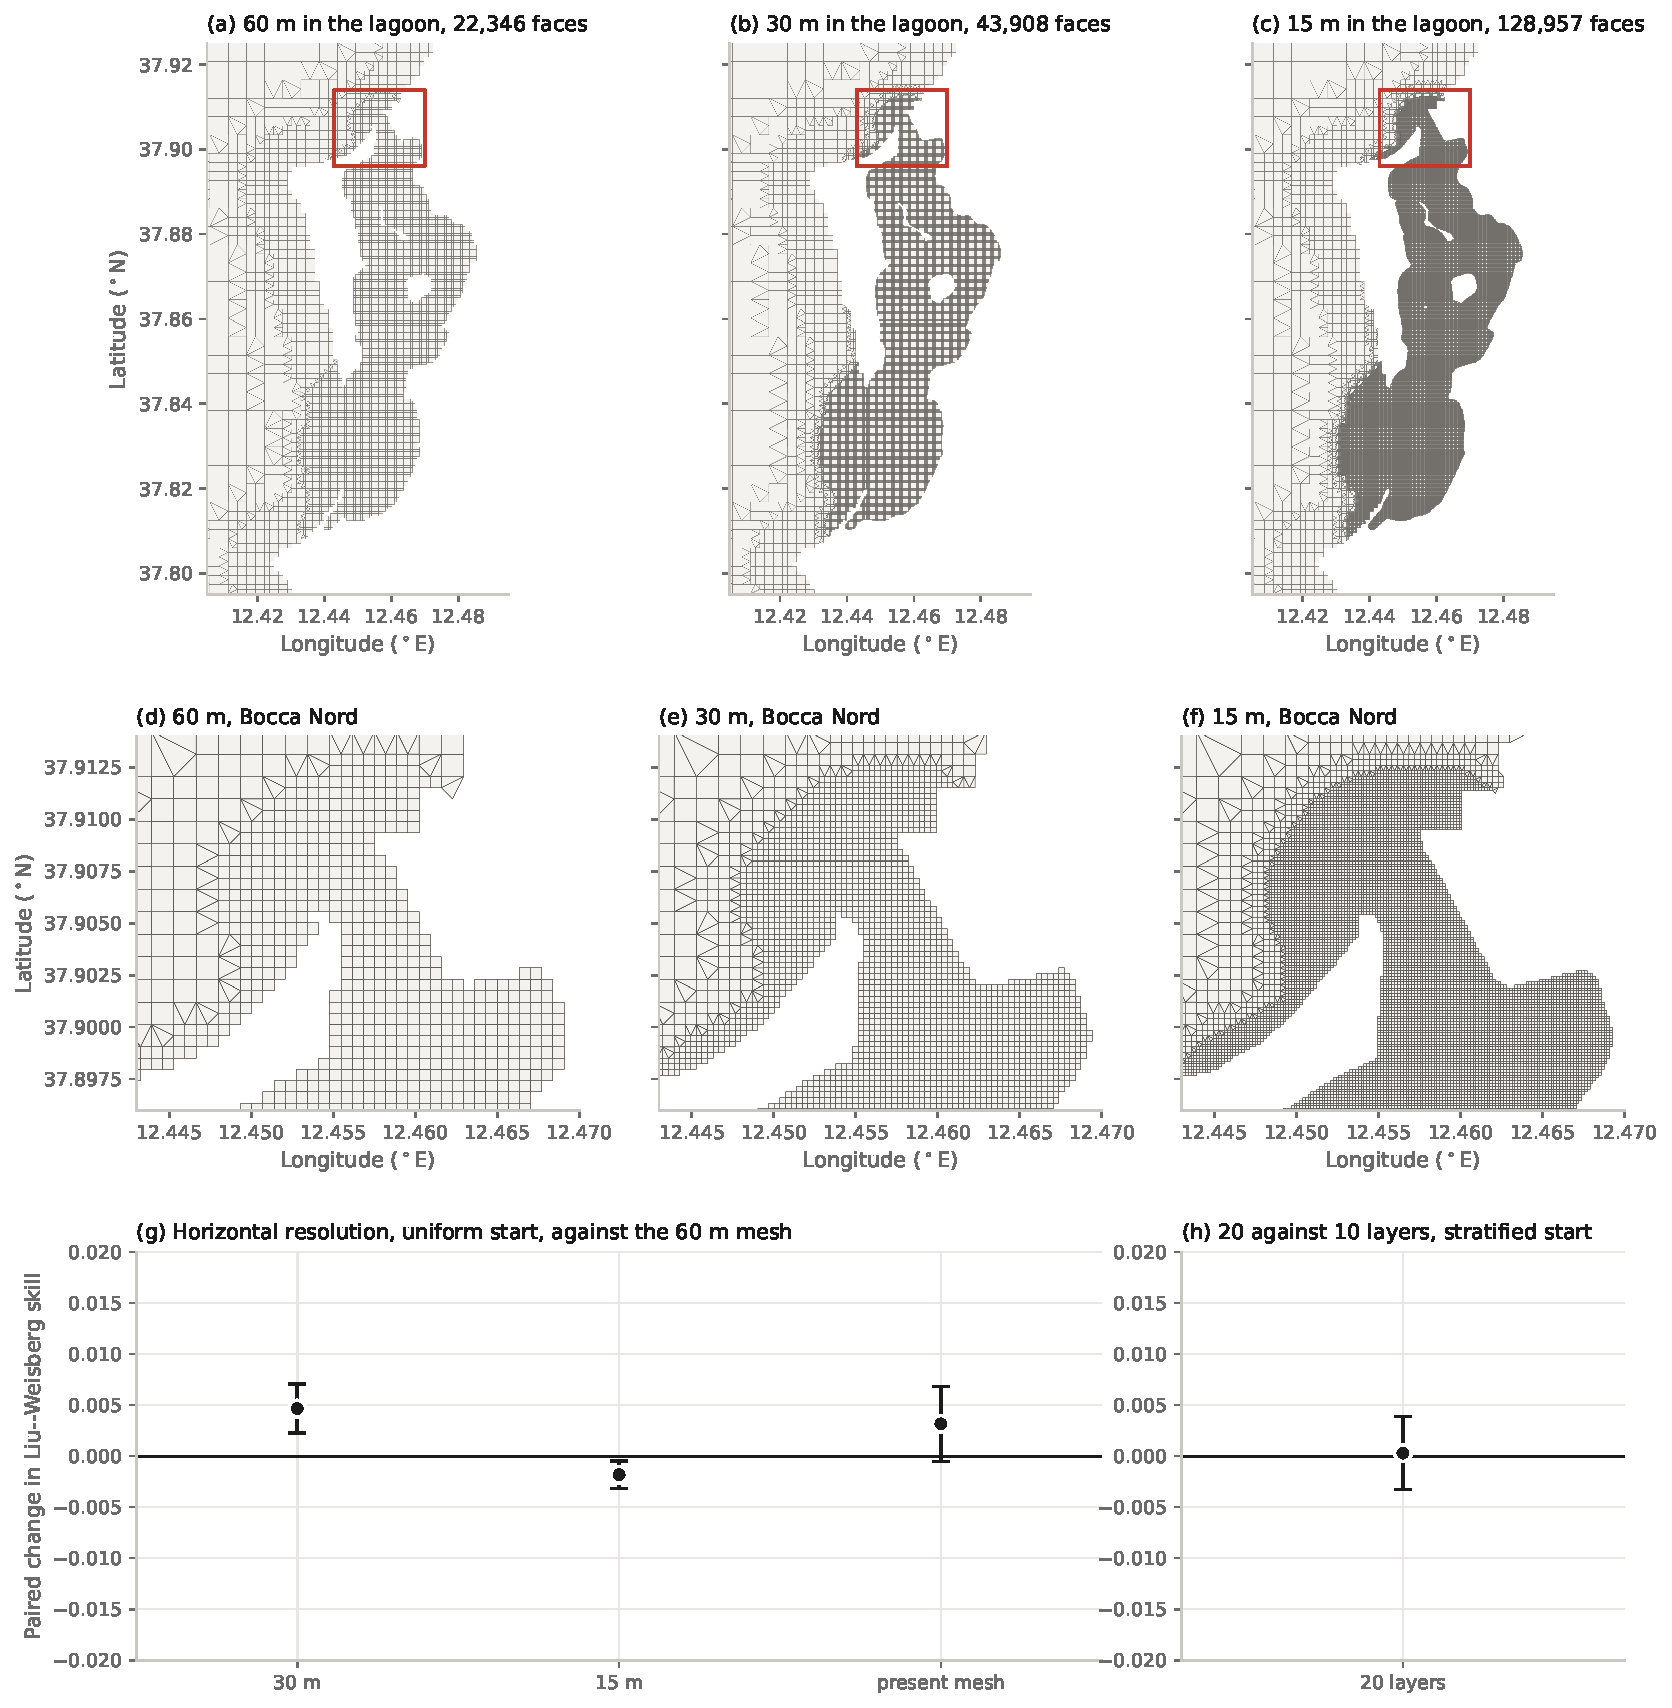
\includegraphics[width=\textwidth]{figS6}
  \caption{Discretisation tests on the uncoupled fixed-bed configuration
  without canopy. (a--c) Quadtree meshes with a cell edge of 60, 30 and 15~m
  in the lagoon and within 500~m of it, and (d--f) the same meshes at the
  northern inlet, Bocca Nord, over the extent of the boxes in (a--c). (g) Paired change in Liu--Weisberg
  skill over the 35 drifters against the 60~m mesh, from the uniform start
  under a Courant limit of 0.5, for the 30 and 15~m meshes and for the present
  mesh carrying the same bed. (h) Paired change from 10 to 20 layers, from the
  stratified start. Error bars give one standard error of the paired
  difference.}
  \label{fig:s_numerics}
\end{figure}

Under the Courant limit of 0.7 used by the ensemble, the uncoupled member started
from the uniform column scored
$0.034 \pm 0.004$ lower on four partitions on the second computer than on eight
on the server, with all 35 drifters worse. Under a limit of 0.5 the same
comparison gave $+0.002 \pm 0.001$ on the present mesh and no difference on the
60~m quadtree mesh.

\section{Restart segments and deployment 4}
\label{sec:s_extra}

A segment of the bare wave-coupled mobile-bed member, restarted on 7~July
without any other change, reproduces the continuous member to within 1.5~mm in
anomaly RMSE at all three stations and to within 0.003 in Liu--Weisberg skill.

Deployment 4 is the one deployment that argues against the canopy, its bare
fixed-bed members scoring 0.68 and 0.69 against 0.48 and 0.50 for its vegetated
ones. It is also a sampling outlier, 0.4~hours in the water over 162~m of
observed path against next-lowest values of 1.9~hours and 723~m. Excluding it
widens the two canopy contrasts on the fixed bed to $+0.148$ and $+0.144$ and
leaves the wave contrasts at $-0.025$ and $-0.029$. In its tracks both
fixed-bed configurations leave to the east and northeast where the observed
drifter went east-southeast.

\section{Online access to the model output}
\label{sec:s_portal}

The model output can be inspected in a web portal hosted on the object storage
of the European Digital Twin of the Ocean platform (EDITO), at
\url{https://minio.dive.edito.eu/oidc-cmartinsjr/wetwise-portal/index.html}.
The portal is a static page served directly from the storage bucket, and it
animates water level, surface velocity and significant wave height over the
simulation window at 30-minute intervals, with the observed and modelled water
level at the gauge stations alongside the map (Fig.~\ref{fig:s_portal}). The
fields were interpolated from the unstructured mesh onto two regular grids, a
base grid of 0.003$^\circ$, about 270~m, over the whole domain and a detail
grid of 0.0005$^\circ$, about 45~m, over the lagoon, which is drawn over the
base grid when the map is zoomed onto the lagoon. The land mask follows the
mesh faces exactly, so that islands smaller than the grid spacing are
retained. The run displayed couples the wave model, a canopy represented as
bed roughness and a mobile bed.

\begin{figure}[H]
  \centering
  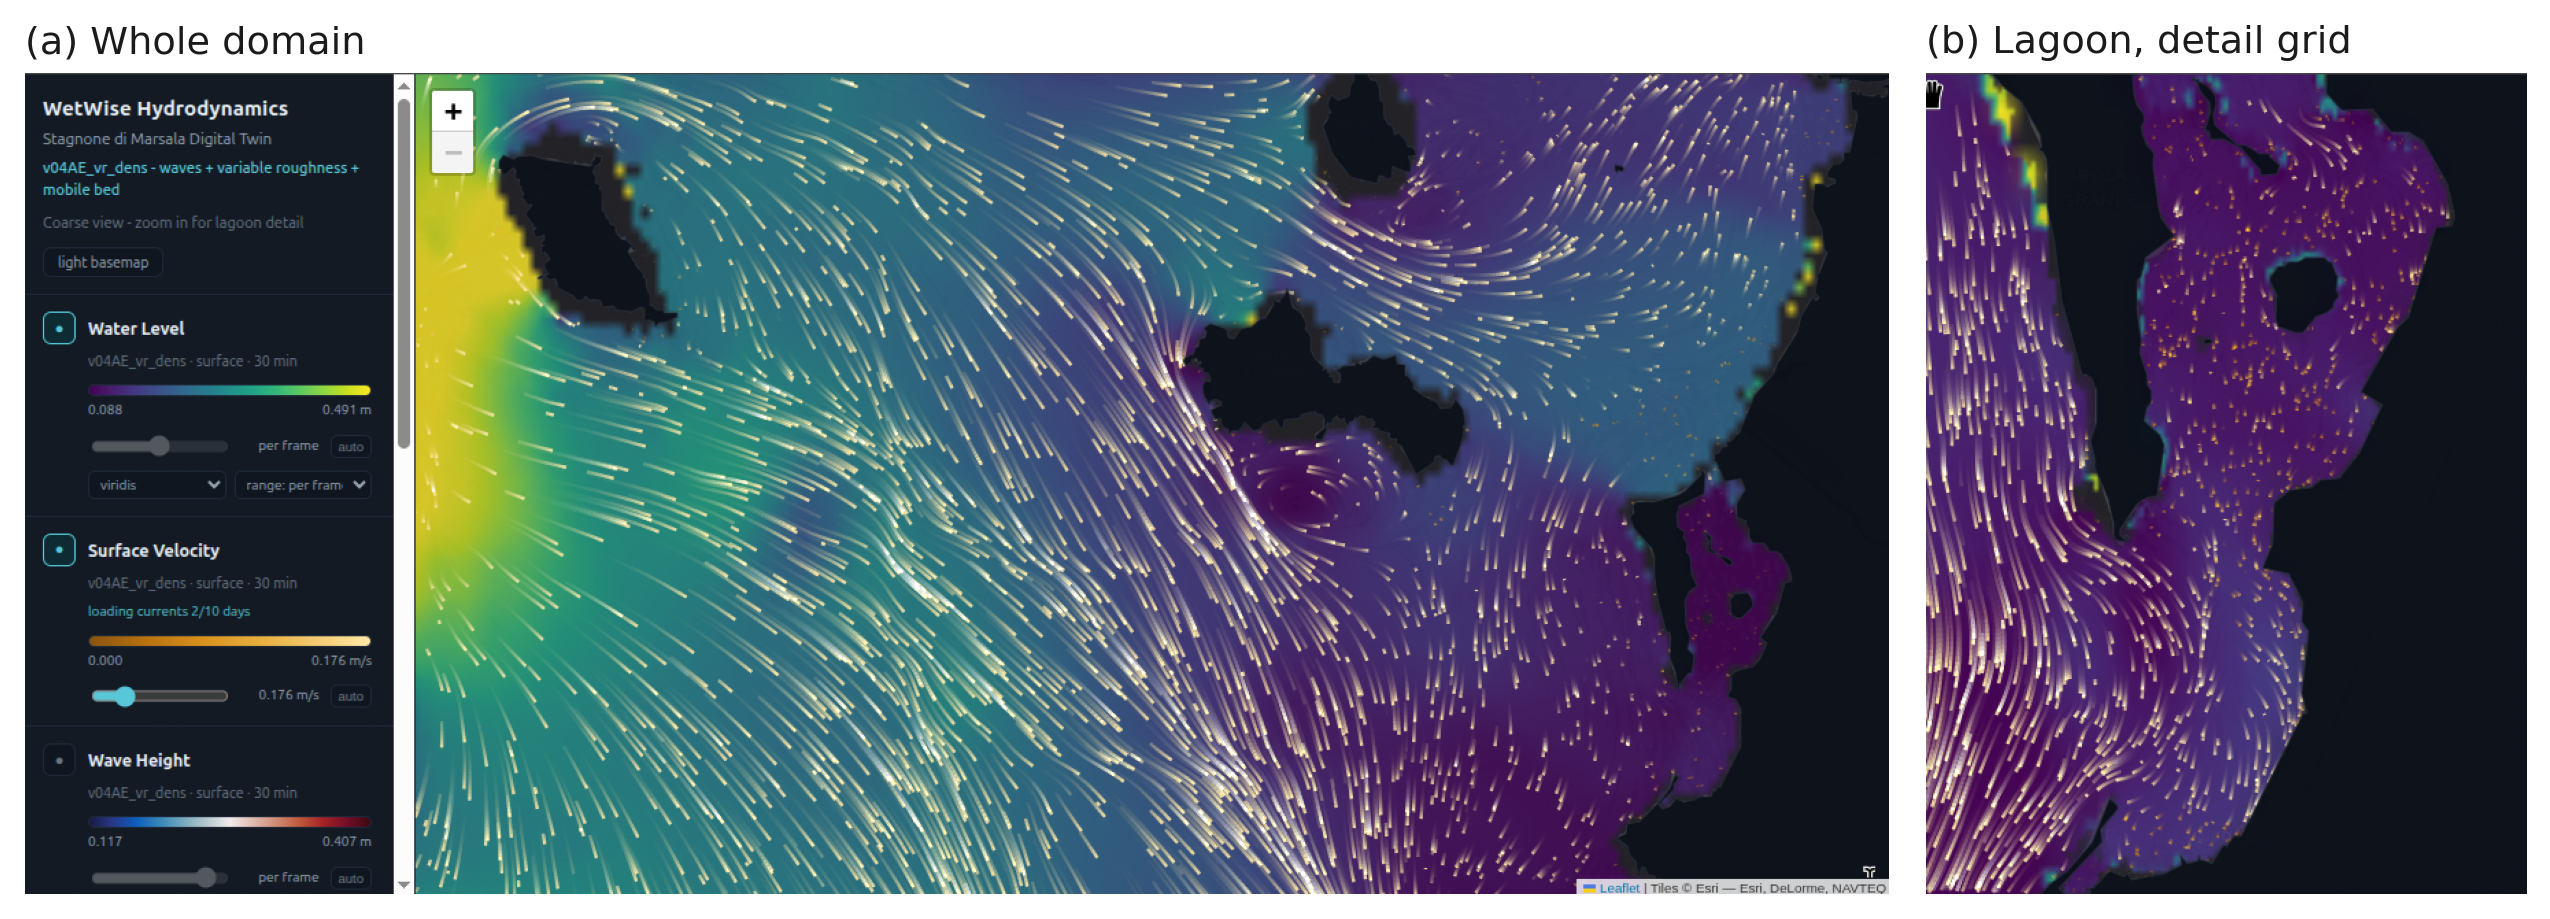
\includegraphics[width=\textwidth]{figS8_portal}
  \caption{Web portal of the model output on the EDITO object storage, showing
  the water level in colour and the surface current as moving particle traces
  at one instant of the simulation window, (a) over the whole domain on the
  base grid, with the layer controls, and (b) over the lagoon on the detail
  grid.}
  \label{fig:s_portal}
\end{figure}

\bibliographystyle{elsarticle-harv}
\bibliography{references}

\end{document}
